\documentclass[../main.tex]{subfiles}

% \title{Abbe sine condition}
% \date{2018-02-05}
% \author{Hongjie Lu}

\begin{document}

	% \maketitle
	% \pagenumbering{gobble}
	% \newpage
	\section{Derivation of Abbe and Herschel condition}
	\begin{figure}[h!]
	  \centering
	  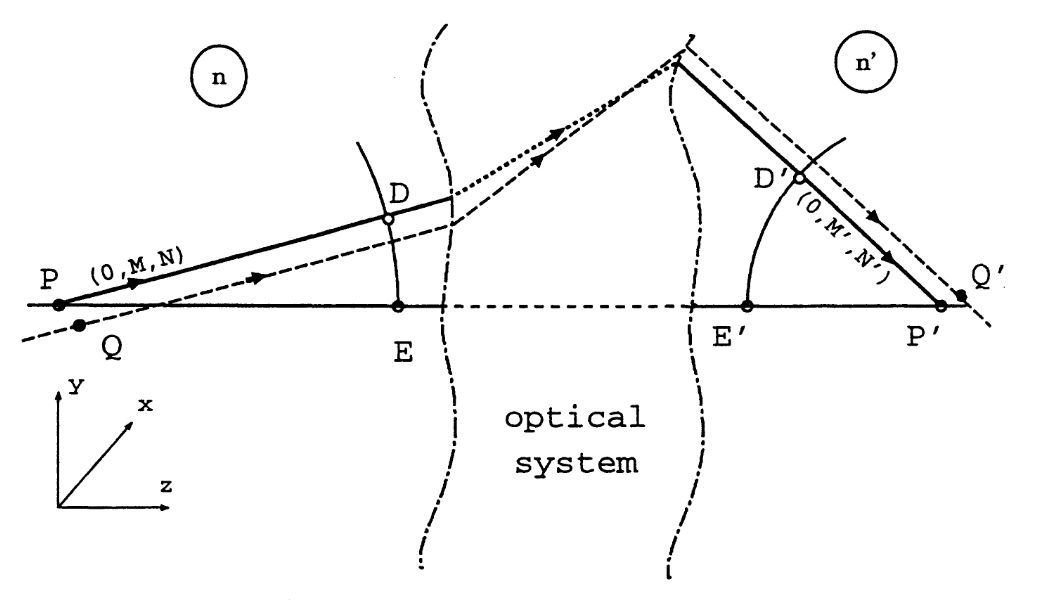
\includegraphics[scale=0.7]{../graphics/Abbe_sine_condition1.png}
	  \caption{Abbe sine condition}
	  \label{fig:abbe}
	\end{figure}
	In figure \ref{fig:abbe} we schematically show an optical system with its entrance and exit pupil located at E and E'. From a pencil of rays leaving the object point P only a certain ray PDD'P' is shown with direction cosines$(0,M,N)$ and $(0,M',N')$ in respectively the object and image space (D and D' are located on the pupil reference spheres). The plane of the drawing is the yz-plane with x=0. We suppose that the pencil of rays is exactly focused at P' (stigmatic imaging). We now want to know how a pencil of rays leacing a neighbouring object Q is focused in image space. According to paraxial optics, the position of an image point Q' derived from the object point Q, which has been subjected to infinitesimal shifts $\delta y$ and $\delta z$ with respect to P, is found by applying the correct (paraxial) magnification factors. The lateral magnification factor is denoted by 
	\begin{equation}
	\beta'=\delta y'/\delta y
	\end{equation}
	and the axial magnification factor is 
	\begin{equation}
	\delta'=\delta z'/\delta z
	\end{equation}
	It can be shown that the relationship between the lateral and axial magnification is given by 
	\begin{equation}
	\delta' = \frac{n'}{n}\beta'^2
	\end{equation}
	It now has to be seen under what condition the image quality of Q' can be equal to the (perfect) quality of P'. To this goal, we take, from the pencil of rays through Q, a particular ray (dashed in the figure) which is parallel to the ray through P shown in the drawing. Physically spoken, we consider this ray to represent a small part of a plane wave with the direction cosines(0,M,N). If the reference point for measuring path length is shifted from P towards Q, the change $\Delta W$ in path of the propagating wave disturbance along the ray from P to P' is given by the scalar product of the ray vector $\vec{s}=(0,M,N)$ and the displacement vector $\delta \vec{r}=(0,\delta{y},\delta{z})$ multiplied with the refractive index of the object space:
	\begin{equation}
	\Delta{W}=-n\delta{\vec{r}}\vec{s}
	\end{equation}
	The minus sign is needed here because a shift of Q in the positive z-direction leads to shorter optical path for the ray along the optical axial.\\
	In the image space, given the image displacement vector $\delta{\vec{r'}}$ and the ray vector $\vec{s'}$, we observe a path difference $\Delta{W'}$ according to 
	\begin{equation}
	\Delta{W'}=-n'\delta{\vec{r'}}\vec{s'}
	\end{equation}
	Equal imaging quality in Q and P(isoplanatism) is obtained when the residual $\delta{W}$ of the path difference in object and image space is zero for arbitary values of the ray vectors of all rays belonging to the object and image space pencils, 
	\begin{equation}
	\delta{W}=\Delta{W}+\Delta{W'}=0
	\end{equation}
	We discern two particular cases:

	\subsection{Abbe sine condition}
	$\delta \vec{r}=(0,\delta{y},0)$\\
	The isoplanatic condition now becomes:\\
	\begin{align}
	&\delta{W_C}=n'\delta{y'}{M'}-n\delta{y}{M}=0\\
	&\delta{W_C}=\left[M'-\frac{nM}{n'\beta'}\right](n'\delta{y'})
	\end{align}
	Here we use the paraxial magnification $\beta'$. This condition, which guarantees the absence of aberration if an infinitesimal lateral excursion off-axis is applied, is generally known as Abbe's sine condition. We have used index C for the aberration because this aberration is called coma.
	\subsection{Herschel condition}
	$\delta \vec{r}=(0,0,\delta{z})$\\
	The isoplanatic condition now becomes:\\
	\begin{align}
	&\delta{W_S}=n'\delta{z'}{N'}-n\delta{z}{N}=0\\
	&\delta{W_S}=\left[N'-\frac{n^2N}{n'^2\beta'^2}\right](n'\delta{z'})
	\end{align}	
	This condition, which guarantees an extended axial range over which the object point can be shifted, is known as Herschel's condition. The subscript S has been used because the aberration which could appear is circularly symmetric spherical aberration.\\
	In general, the constant pathlength difference $n'\delta z'-n\delta z$ encountered for the axial ray (N=N'=1) is subtracted from the expression above and we obtain:
	\begin{equation}
	\delta{W_S}=\left[(N'-1)-\frac{n^2(N-1)}{n'^2\beta'^2}\right](n'\delta{z'})=0
	\end{equation}
	\subsection{Comparsion between Abbe and Herschel}
	Abbe's sine condition is a prerequisite for an opticla system which needs to image an extended flat object, e.g., for a photographic camera objective, a reduction objective but also for a microscope objective or an astronomical telescope.\\
	Herschel's condition is required when a system needs to operate at different magnifications, e.g., a narrow field telescope for both remote and close observation.\\
	Unfortunately, both conditions seriously conflict when the numerical aperture becomes high. A particular case arises when $\beta'=\pm\frac{n}{n'}$, a case which reduces to unit magnification when $n=n'$; here, both conditions can be satisfied simultaneously. In most applications, it is the sine condition which will prevail because otherwise the useful lateral or angualr image field would become unacceptably small.
	\subsection{Reference}
	\begin{itemize}  
	\item Braat, J.: The Abbe sine condition and related imaging conditions in geometrical optics. In Proc. SPIE, checked on 11/7/2016.
	\end{itemize}
	\section{Modified sine relationship for spherical mirror at grazing incidence}
	\begin{figure}[h!]
	  \centering
	  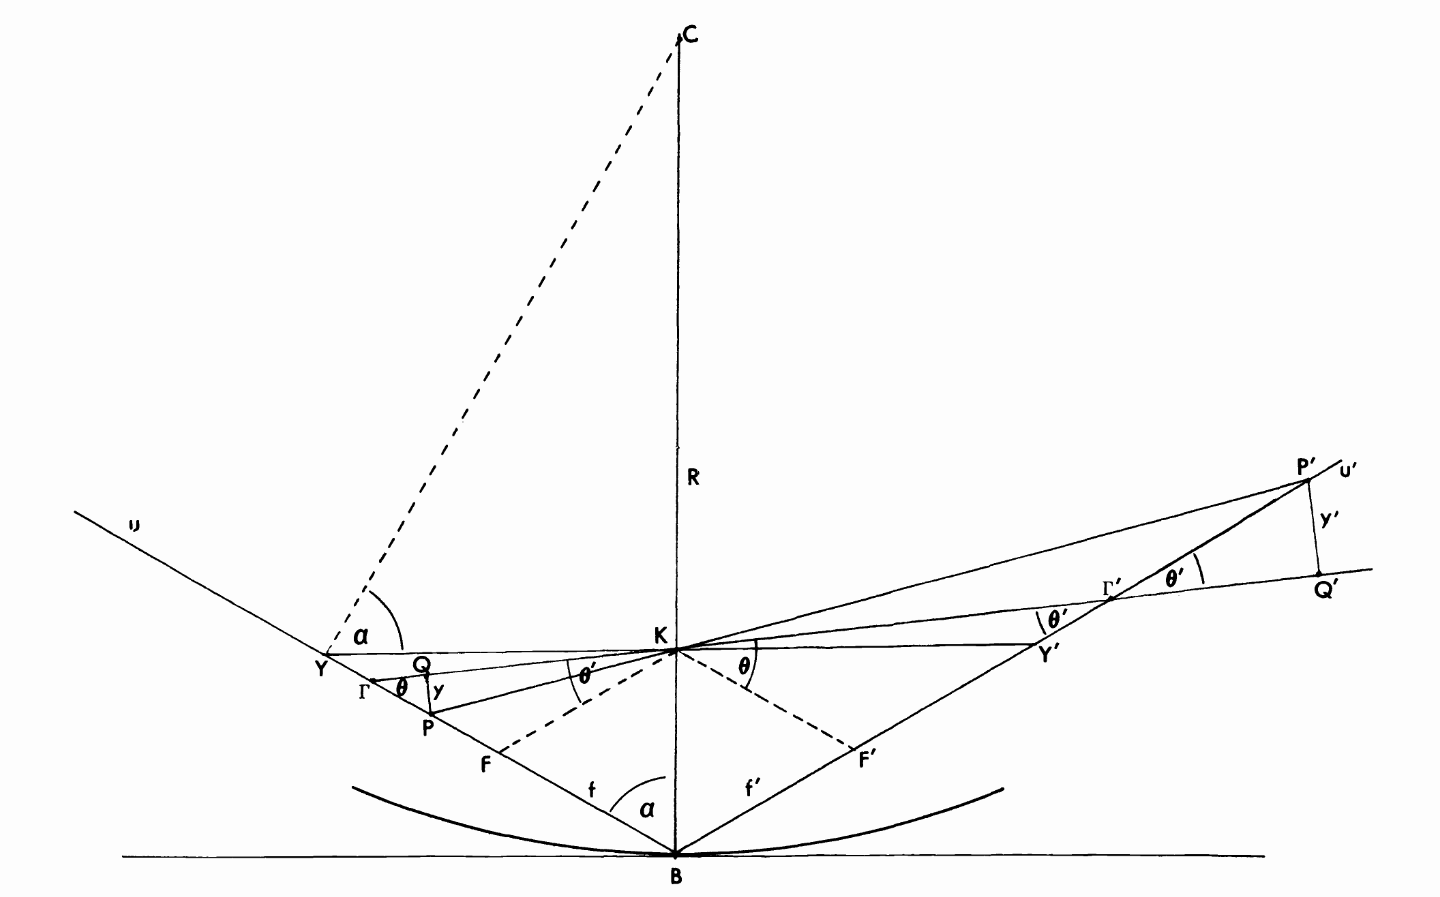
\includegraphics[scale=0.4]{../graphics/Abbe_sine_condition2.png}
	  \caption{Ray construction for reflection at grazing incidence leading to a modified sine condition.}
	  \label{fig:modified abbe}
	\end{figure}
	In figure\ref{fig:modified abbe} a concave reflector with its apex at B and of radius R has points Y and Y' which make CY and CY' perpendicular to the incoming and outgoing ray direction $\mu$ respectively. The center of perspective is at K. $CK=Rsin^2\alpha$ and consequently $KB=R(1-sin^2\alpha$ which is very small for the case of grazing incidence where $\alpha$ approaches $90^{\circ}$.\\
	In the figure, the distance $PB=p$ the object distance and $BP'=q$ the image distance then since the triangles PFK and KF'P' are similiar, the ratio of corresponding sides results in
	\begin{align}
	&\frac{p-f}{f'}=\frac{f}{q-f'}\\
	&(p-f)(q-f')=ff'\label{eq1}\\
	\end{align}
	which is recognized as Newton's Equation in optics. By substituting $f'=f=\frac{Rsini}{2}$, the well known focal length in the meridian plane for grazing incidence, where $i=90^{\circ}-\alpha$ and R is the radius of curvature of the reflecting surface, the equation reduces to
	\begin{equation}
	\frac{1}{p}+\frac{1}{q}=\frac{2}{Rsini}
	\end{equation}
	the equation commonly used to determining image formation at grazing angles of incidence in the meridian plane.\\
	For point P in figure the distance $(p-f)$ and $(q-f)$is given by
	\begin{align}
	&(p-f)=PF=\Gamma F-\Gamma P\\
	&(q-f)=F'P'=F'\Gamma'+\Gamma'P'
	\end{align}
	By construction
	\begin{align}
	&PQ=y=\Gamma Psin\theta\\
	&P'Q'=y'=\Gamma'P'sin\theta'\\
	&\frac{\Gamma F}{sin\theta'}=\frac{f}{sin\theta}\\
	&\frac{\Gamma'F'}{sin\theta}=\frac{f}{sin\theta'}
	\end{align}
	Substitution in Eq. \ref{eq1} yields
	\begin{align}
	&f^2=(\Gamma F-\Gamma P)(\Gamma' F'-\Gamma' P')\\
	&f^2=\left(f\frac{sin\theta'}{sin\theta}-\frac{y}{sin\theta}\right)\left(f\frac{sin\theta}{sin\theta'}+\frac{y'}{sin\theta'}\right)
	\end{align}
	and get the modified sine condition for grazing incidence optics
	\begin{equation}
	y'sin\theta'-ysin\theta=\frac{yy'}{f}
	\end{equation}
	\subsection{Reference}
	\begin{itemize}  
	\item Mcgee, J. F.; Keski-Kuha, Ritva A. M. (1986): A Modified Sine Condition for Grazing Incidence Optics. In Proc. SPIE, p. 640, checked on 7/19/2016.
	\end{itemize}
	\section{generalized sine condition for Wolter type II and WS telescope}
\end{document}